%Copyright 2019 Christopher M. Jermaine (cmj4@rice.edu) and Risa B. Myers (rbm2@rice.edu)
%
%Licensed under the Apache License, Version 2.0 (the "License");
%you may not use this file except in compliance with the License.
%You may obtain a copy of the License at
%
%    https://www.apache.org/licenses/LICENSE-2.0
%
%Unless required by applicable law or agreed to in writing, software
%distributed under the License is distributed on an "AS IS" BASIS,
%WITHOUT WARRANTIES OR CONDITIONS OF ANY KIND, either express or implied.
%See the License for the specific language governing permissions and
%limitations under the License.
%===============================================================

\documentclass[aspectratio=169]{beamer}
\mode<presentation> 
{
\usetheme[noshadow, minimal,numbers,riceb,nonav]{Rice}
\usefonttheme[onlymath]{serif}
\setbeamercovered{transparent}
}
\useinnertheme{rectangles}

\usepackage[english]{babel}

\usepackage{amsmath}
\usepackage{mathptmx}
\usepackage{helvet}
\usepackage{courier}
\usepackage[T1]{fontenc}
\usepackage{trajan}
\usepackage{ textcomp }
\usepackage{listings}

\newenvironment{noindentitemize}
{ \begin{itemize}
 \setlength{\itemsep}{1.5ex}
  \setlength{\parsep}{0pt}   
  \setlength{\parskip}{0pt}
 \addtolength{\leftskip}{-2em}
 }
{ \end{itemize} }

\newenvironment{noindentitemize2}
{ \begin{itemize}
  \setlength{\itemsep}{0ex}
  \setlength{\parskip}{0pt}
  \setlength{\parsep}{0pt}   
  \addtolength{\leftskip}{-2em}  }
{ \end{itemize} }

\lstnewenvironment{SQL}
  {\lstset{
        aboveskip=5pt,
        belowskip=5pt,
        escapechar=!,
        mathescape=true,
        upquote=true,
        language=SQL,
        basicstyle=\linespread{0.94}\ttfamily\footnotesize,
        morekeywords={WHILE, DO, END},
        deletekeywords={VALUE, PRIOR},
        showstringspaces=true}
        \vspace{0pt}%
        \noindent\minipage{0.47\textwidth}}
  {\endminipage\vspace{0pt}}
  
\newcommand{\LIKES}{\textrm{LIKES}} 
\newcommand{\FREQUENTS}{\textrm{FREQUENTS}} 
\newcommand{\SERVES}{\textrm{SERVES}} 
\newcommand{\CAFE}{\textrm{CAFE}} 
\newcommand{\COFFEE}{\textrm{COFFEE}} 
\newcommand{\DRINKER}{\textrm{DRINKER}} 
\newcommand{\ALLPEEPS}{\textrm{ALLPEEPS}} 
\newcommand{\ALLCOMBOS}{\textrm{ALLCOMBOS}} 


\setbeamerfont{block body}{size=\tiny}

%===============================================================%

\title[]
{Tools \& Models for Data Science}

\subtitle{Generalized Linear Models}

\author[]{Chris Jermaine \& Risa Myers}
\institute
{
  Rice University 
}

\date[]{}

\subject{Beamer}

\begin{document}

\begin{frame}
 \titlepage
\end{frame}

%***********************************************************
\begin{frame}{Last Class: Classical Linear Regression}
\begin{itemize}
\item LR in closed form
			$$\hat{r} = (\textbf{X}^{\textrm{T}}\textbf{X})^{-1}\textbf{X}^{\textrm{T}}\textbf{y}$$

\item LR using Gradient Descent
\begin{itemize}
\item Using the Mean Squared Error Loss function:
	$$\frac{\sum_i(y_i - x_i \cdot r)^2}{n}$$

\end{itemize}
\item Introduction to issues with using LR to handle categorical data
\end{itemize}
     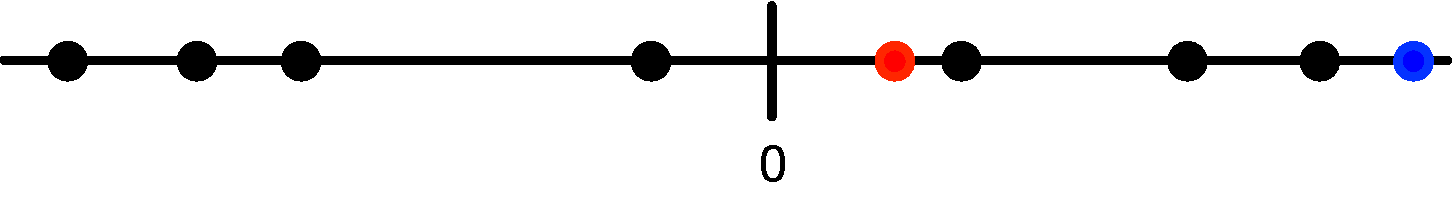
\includegraphics[width=1\textwidth]{lectLR/yesNoCases.pdf} 
\end{frame}
%***********************************************************
\begin{frame}{Linear Regression: Generative Statistical Model with Normal Error}

\begin{columns}
\begin{column}{0.5\textwidth}
\begin{center}Data and LR line
\end{center}
     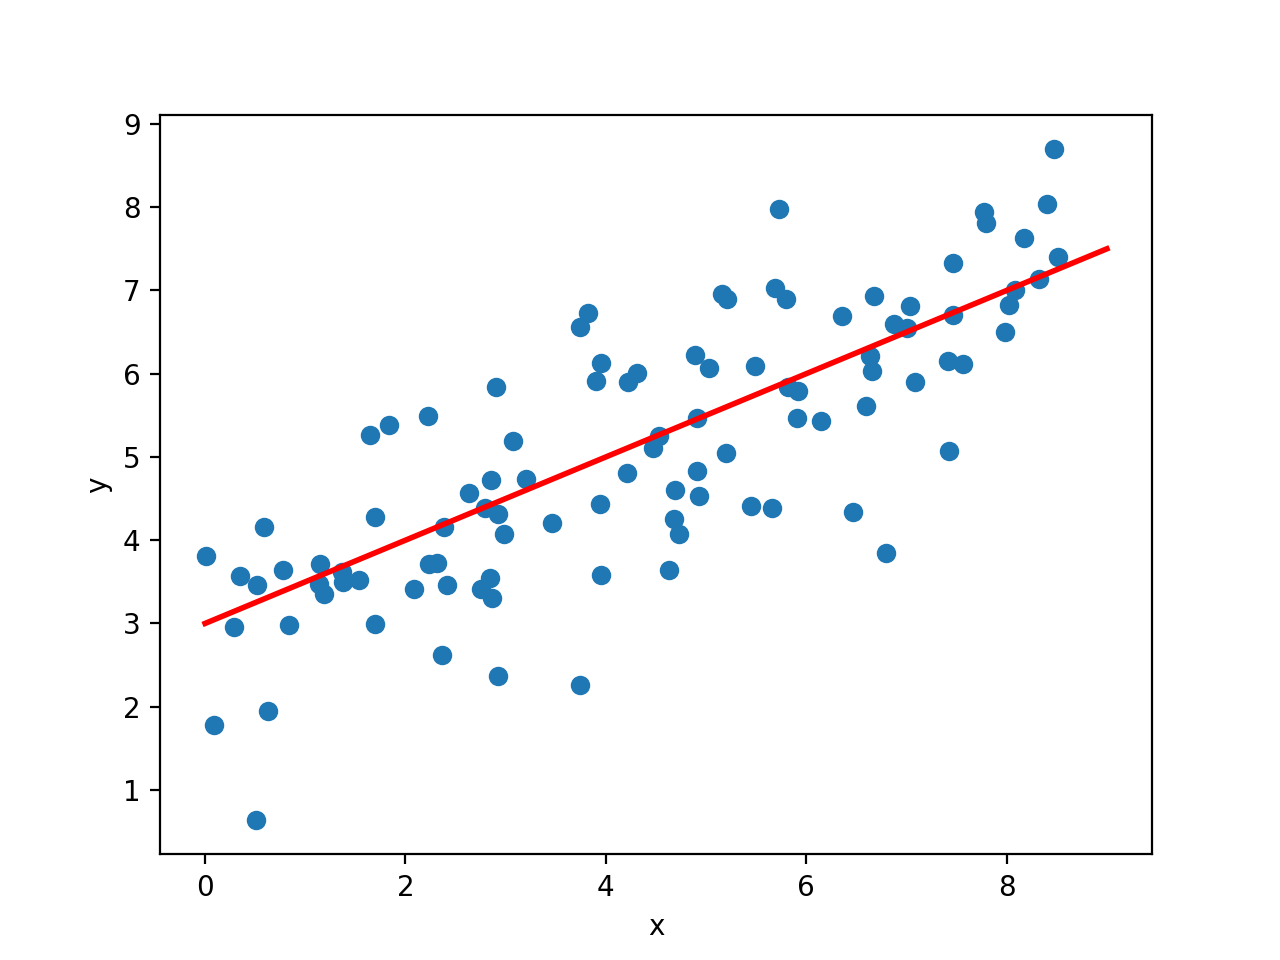
\includegraphics[width=1\textwidth]{lectGLM/LRgenmodel1.png} 
 \end{column}
\begin{column}{0.5\textwidth}
\begin{center}Histogram of error
\end{center}

     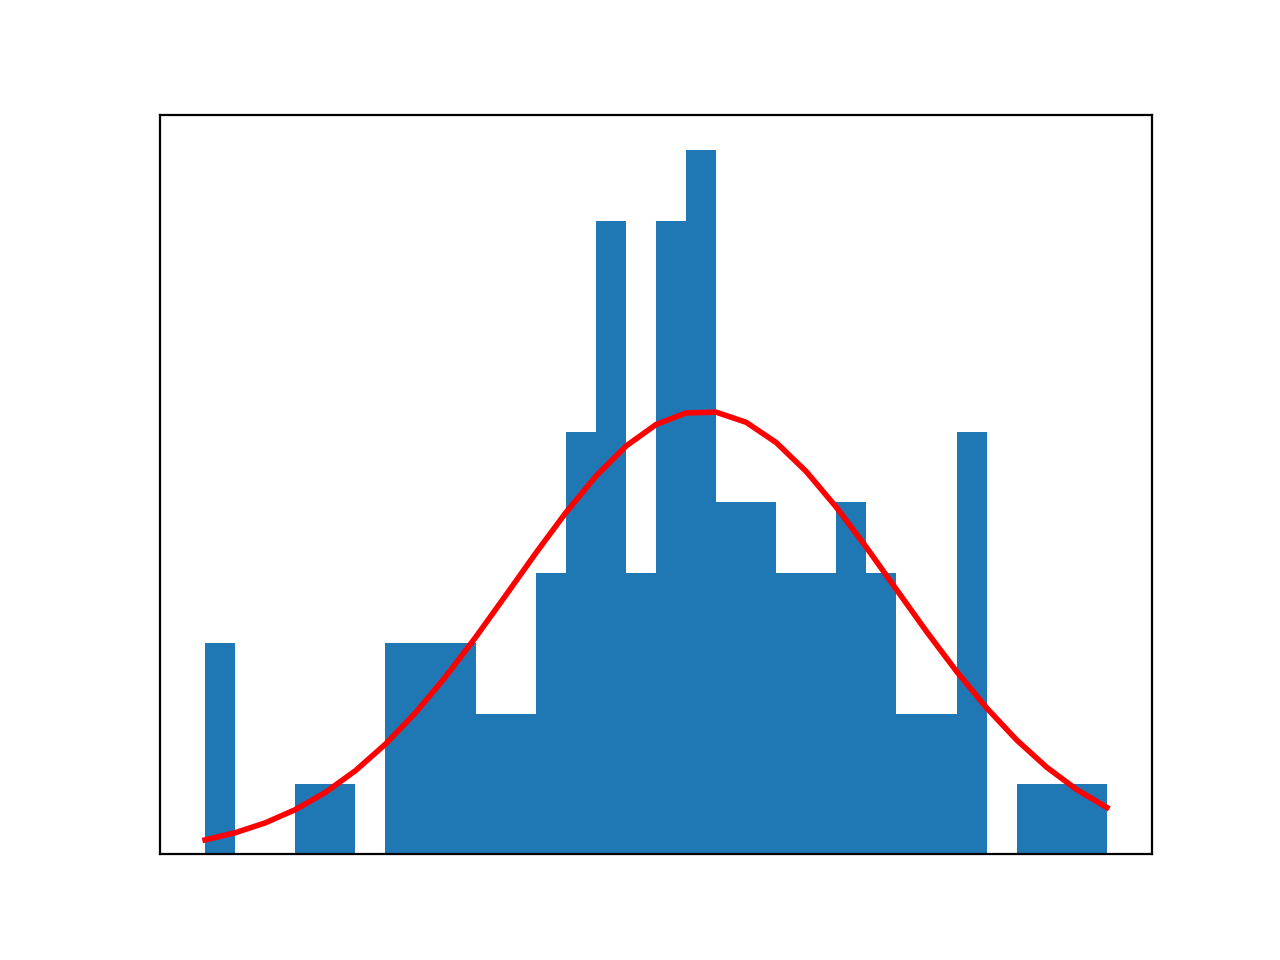
\includegraphics[width=1\textwidth]{lectGLM/LRgenmodelError.png} 
\end{column}
 \end{columns}

\end{frame}

%***********************************************************
\begin{frame}{Where is the Error?}

\begin{columns}
\begin{column}{0.5\textwidth}
\begin{center}Residuals
\end{center}
     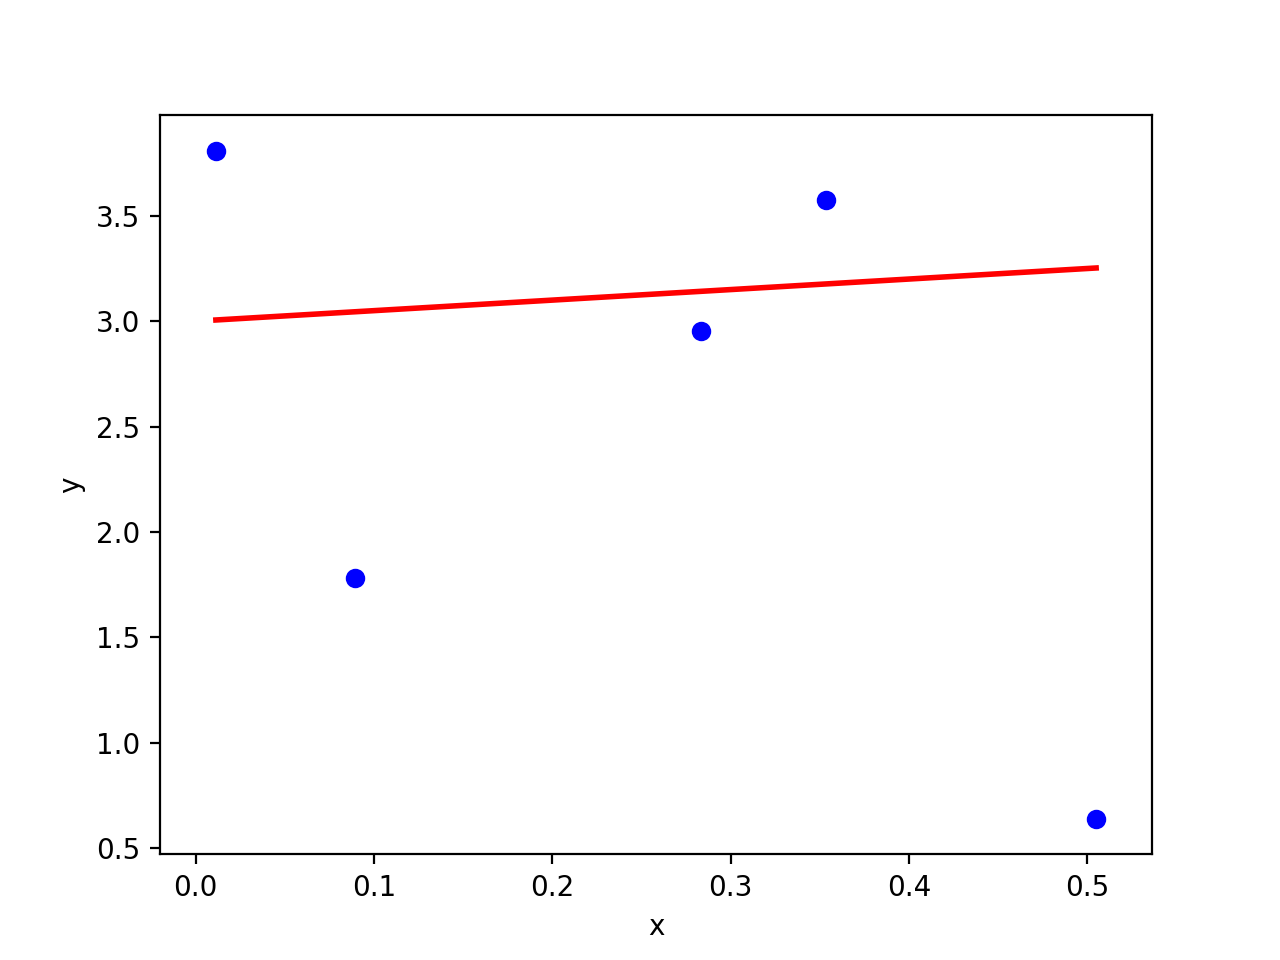
\includegraphics[width=1\textwidth]{lectGLM/LRgenmodelResidual.png} 
 \end{column}
\begin{column}{0.5\textwidth}
\begin{center}
\end{center}

\end{column}
 \end{columns}

\end{frame}

%***********************************************************
\begin{frame}{Probabilistic Interpretation of Classic LR}

	\begin{itemize}
	\item Given $x_i$, let $y_i \sim \textrm{Normal} (x_i \cdot r, \sigma^2)$ % if there were no error, \sigma^2 would be 0
	\item Where we treat $x_i \cdot r$ as the expected value of the regression coefficients and the features of $x$
	\item Then, assuming iid data, the likelihood of data set is $\prod_i \textrm{Normal} (y_i | x_i \cdot r, \sigma^2)$
	\item We can replace the Normal function with its PDF
	$$LH(x_i) = \prod_i \frac{1}{\sqrt{2\pi\sigma^2}} 
                e^{-\frac{(y_i - x_i \cdot r)^2}{2\sigma^2}}$$
	\end{itemize}
\end{frame}

%***********************************************************
\begin{frame}{Probabilistic Interpretation of Classic LR}
	$$LH(x_i) = \prod_i \frac{1}{\sqrt{2\pi\sigma^2}} 
                e^{-\frac{(y_i - x_i \cdot r)^2}{2\sigma^2}}$$

	\begin{itemize}
	\item Take the log of this function to get the Log likelihood  
	$$LLH \propto \sum_i -\frac{(y_i - x_i \cdot r)^2}{2\sigma^{2}}$$
	\item And an MLE over $r$ is going to try to maximize
	$$  -\sum_i (y_i - x_i \cdot r)^2$$
	\item Same loss function as LR, when divided by $n$
	\item This looks a lot like minimizing the squared loss
	\item But: note the negative sign!
	\begin{itemize}
		\item Because we are maximizing instead of minimizing, so invert the function
	\end{itemize}
	\end{itemize}
\end{frame}
%***********************************************************
\begin{frame}{People Noticed This a Long Time Ago}

\begin{itemize}
\item And wondered:
\item Can I use other error models (besides Normal error) with LR?
\item Answer, naturally, is yes!
\end{itemize}
\end{frame}
%***********************************************************
\begin{frame}{Generalized Linear Models (GLM)}

\begin{itemize}
\item Generalization of LR
\item Allows error to be generated by a wide variety of distributions
\item In particular, any in the ``exponential family''
\end{itemize}
\end{frame}
%***********************************************************
\begin{frame}{Which Distributions are in the Exponential Family?}

\begin{itemize}
\item[?]
\end{itemize}
\end{frame}
%***********************************************************
\begin{frame}{Which Distributions are in the Exponential Family?}

\begin{itemize}
\item Normal
\item Bernoulli
\item Exponential
\item Chi-squared
\item Dirichlet
\item Poisson
\item ...
\item[?] What determines if a distribution is in the Exponential Family? % it can be written in a particular canonical form
\end{itemize}
\end{frame}

%***********************************************************
\begin{frame}{When is a Distribution in the Exponential Family?}

\begin{itemize}
\item Any probability distribution that can be written in this canonical form:
$$p (y | \theta) = b (y) \exp (\theta T(y) - f (\theta))$$
\item  $\theta$ are the natural parameters
\item  $y$ is the output
\item  $b$ and $T$ are some arbitrary functions
\item  $f$ is some function of $\theta$
\end{itemize}
% Uniform - non exponential
\end{frame}
%***********************************************************
\begin{frame}{Example: Normal}

\begin{itemize}
\item Assume the variance is 1 (for simplicity): % eliminates sigma 
% this is just the Normal PDF
\begin{align}
p (y | \mu) &= \frac{1}{\sqrt{2 \pi}} \exp (-\frac{1}{2} (y -\mu)^2) \nonumber \\
	&= \frac{1}{\sqrt{2 \pi}} \exp (- \frac{1}{2}y^2 + y \mu - \frac{1}{2}\mu^2) \nonumber \\
	&= \frac{1}{\sqrt{2 \pi}} \exp (-\frac{1}{2}y^2) \exp (\mu y - \frac{1}{2}\mu^2) \nonumber
\end{align}
\item Which is the Normal distribution in canonical form
\end{itemize}
\end{frame}
%***********************************************************
\begin{frame}{Example: Normal}

\begin{itemize}
\item If variance is 1 (for simplicity):
\begin{align}
p (y | \mu) = \frac{1}{\sqrt{2 \pi}} \exp (-\frac{1}{2}y^2) \exp (\mu y - \frac{1}{2}\mu^2) \nonumber
\end{align}
\item Recall, exponential family distribution that can be written as:
$$p (y | \theta) = b (y) \exp (\theta T(y) - f (\theta))$$
\item So we have:
        \begin{itemize}
	\item $\theta$ is $\mu$
	\item $f(\theta)$ = $\frac{1}{2}\theta^2$
	\item $T (y)$ is $y$
	\item $b (y)$ is $\frac{1}{\sqrt{2 \pi}} \exp (-\frac{1}{2}y^2)$
	\end{itemize}
\end{itemize}
\end{frame}
%***********************************************************
\begin{frame}{This Brings Us to GLMs}

\begin{itemize}
\item Say we have a prediction problem where:
\end{itemize}
\begin{enumerate}
\item  We want to predict output $\boldsymbol{y}$ from an input vector $\boldsymbol{x}$
\item  It is natural to assume randomness/error/uncertainty on $\boldsymbol{y}$ is produced by some exponential family
\item  The exponential family parameter $\boldsymbol{\theta}$ is \textbf{linearly related} to $x$%: that is, assuming $x$ is vector-valued:
%$$\theta = \sum_j x_j \times r_j$$
{\small
\[
\boldsymbol{\theta} = X\boldsymbol{r} =  \begin{bmatrix} 
 \rule[.025in]{.75in}{0.5pt}	&\boldsymbol{x_1}  & \rule[.025in]{.75in}{0.5pt}	\\
	& $\vdots$ & 	\\
\rule[.025in]{.75in}{0.5pt}		&\boldsymbol{x_i} & \rule[.025in]{.75in}{0.5pt}		\\
	&$\vdots$  & 	\\
 \rule[.025in]{.75in}{0.5pt}	&\boldsymbol{x_n}  & \rule[.025in]{.75in}{0.5pt}	\\
\end{bmatrix} \times
 \begin{bmatrix} 
	 & & 	\\
	 &   & 	\\
	 &   & 	\\
	 & \boldsymbol{r} & 	\\
	 &   & 	\\
	 &  & 	\\
	 & & 	\\
\end{bmatrix} 
= \begin{bmatrix} 
	 & x_1r_1  & 	\\
	 & & \\
	 &  $\vdots$ & 	\\
	 & x_ir_i & 	\\
	 & $\vdots$ & 	\\
	 & x_n r_n& 	\\
\end{bmatrix} 
\]
}
\end{enumerate}
\begin{itemize}
\item Then this is known as an instance of a ``generalized linear model'' 
\item E.g.: We might use a Poisson distribution, to predict an arrival time with some error or uncertainty
\end{itemize}
\end{frame}
%***********************************************************
%\begin{frame}{TBD}
%
%\begin{itemize}
%\item We have a definition of $\boldsymbol{\theta}$, given our data 
%$$\boldsymbol{\theta} = X\boldsymbol{r}$$
%\item However, $\boldsymbol{r}$ is still unknown
%\item We want the LLH of the data set
%\item LLH(X) is a function of $\boldsymbol{r}$
%\end{itemize}
%\end{frame}
%***********************************************************
\begin{frame}{LLH Of Data Produced by GLM}

\begin{itemize}
\item From GLM definition, likelihood of the data set is: % product of iid probabilities
$$\Pi Pr(y_i|\boldsymbol{\theta}) = \prod_i b(y_i) \exp (\theta_i T(y_i) - f(\theta_i))$$
\item Where $\theta_i$ is produced by the dot product of the feature vector and the regression coefficients
%\item Substituting $x_{i,j} \times r_{i,j}$ for $\theta_i$, we have:
$$\prod_i b(y_i) \exp \left(T(y_i) \Big(X_i \cdot \boldsymbol{r}\Big) - f\Big(X_i \cdot \boldsymbol{r}\Big) \right)$$
\item Take the log to get the LLH: % \pi becomes \sum; b(y_i) becomes log b(y_i)
$$\sum_i \left( \log b(y_i) + T(y_i) X_i \cdot \boldsymbol{r} \Big) - f\Big(X_i \cdot \boldsymbol{r}  \Big)\Big) \right)$$
\end{itemize}
\end{frame}
%***********************************************************
\begin{frame}{Then, For Any Member of Exponential Family...}

\begin{itemize}
\item We have
$$LLH = \sum_i \left( \log b(y_i) + T(y_i) X_i \cdot \boldsymbol{r} \Big) - f\Big(X_i \cdot \boldsymbol{r}  \Big)\Big) \right)$$

\item Maximize to learn the model
\begin{itemize}
\item Take the derivative and set to 0, or
\item Use Gradient Descent to determine $\boldsymbol{r}$
\end{itemize}
\item Let's look at another example:
\end{itemize}
\end{frame}
%***********************************************************
\begin{frame}{Example: Bernoulli}

\begin{itemize}
\item Recall the Bernoulli distribution, which models a coin flip
\item \{Tails, Heads\} = \{0, 1\}
\item First, write Bernoulli as:
\begin{align}
p (y | p) = &p^y \times (1 - p)^{(1 - y)} \nonumber \\
	= &\exp (y \log p + (1 - y) \log (1 - p)) \nonumber \\
	= &\exp ((\log p - \log (1 - p)) y + \log (1 - p)) \nonumber
\end{align}
% do some algebra
\item $p$ is the natural parameter for Bernoulli
\end{itemize}
\end{frame}
%***********************************************************
\begin{frame}{Example: Bernoulli}

\begin{itemize}
\item First, write Bernoulli in exponential form as:
\begin{align}
p (y | p) = &p^y \times (1 - p)^{(1 - y)} \nonumber \\
	= &\exp (y \log p + (1 - y) \log (1 - p)) \nonumber \\
	= &\exp ((\log p - \log (1 - p)) y + \log (1 - p)) \nonumber
\end{align}
\item Recall, exponential family distribution that can be written as:
$$p (y | \theta) = b (y) \exp (\theta T(y) - f (\theta))$$
\item So, for Bernoulli, we have:
	\begin{itemize}
	\item $\theta$ is $(\log p - \log (1 - p))$ = $\log (\frac{p}{1 - p})$
	\item $f(\theta)$ = $-\log (1 - p) = \log (1 + e^\theta)$ 
	\item $T (y)$ is $y$
	\item $b (y)$ is $1$ % there is no b function here, so set it to 1
	\end{itemize}
\item Here $\theta$ is the ``natural parameter'' of the distribution
\end{itemize}
\end{frame} % so Bernoulli is a GLM
%***********************************************************
\begin{frame}{Example: Logistic Regression}

\begin{itemize}
\item Plugging in the Bernoulli expression into the LLH
\item LLH for GLM is:
$$\sum_i \left( \log b(y_i) + T(y_i)X_i \cdot \boldsymbol{r} \Big) - f \Big(X_i \cdot \boldsymbol{r} \Big) \Big) \right)$$
\item For Bernoulli data have:
	\begin{itemize}
	\item $\theta$ is $(\log p - \log (1 - p))$ or $\log (p / (1 - p))$
	\item $f(\theta)$ = $-\log (1 - p) = \log (1 + e^\theta)$ 
	\item $T (y)$ is $y$
	\item $b (y)$ is $1$
	\end{itemize}
\item Substituting in these values (and letting $\theta_i = X_i \cdot \boldsymbol{r}$)
$$\sum_i \log 1 + y_i (X_i \cdot \boldsymbol{r}) - \log (1 + e^{X_i \cdot \boldsymbol{r}})$$
\end{itemize}
\end{frame}
%***********************************************************
\begin{frame}{Example: Logistic Regression}

$$\sum_i \log 1 + y_i (X_i \cdot r) - \log (1 + e^{X_i \cdot \boldsymbol{r}})$$
\begin{itemize}
\item Dropping the $\log 1$ and maximizing wrt $\boldsymbol{r}$ gives us logistic regression
\item[?] Why can we drop the $\log 1$
% can drop the log 1 because it's a constant 
\item How to maximize?
\begin{itemize}
\item Use any method we've discussed
\item Typically using gradient \textbf{ascent} % 
\begin{itemize}
\item Ascent, not descent because we are typically using an MLE, which is a maximization problem
\end{itemize}
\end{itemize}
\end{itemize}
\end{frame}
%***********************************************************
\begin{frame}{Example: Logistic Regression}

$$LLH = \sum_i \log 1 + y_i (X_i \cdot \boldsymbol{r}) - \log (1 + e^{X_i \cdot \boldsymbol{r}})$$
\begin{itemize}
\item How to predict?
\begin{itemize}
\item Given $\boldsymbol{r}, X_i$ make a prediction for unknown $y_i$, choose $y_i$ to maximize LLH
\item That is, choose $y_i$ to match sign of $X_i \cdot \boldsymbol{r}$
\item Note that no closed form exists
\end{itemize}
\end{itemize}
\end{frame}
%***********************************************************
\begin{frame}{Prediction using Logistic Regression}

$$LLH = \sum_i  y_i (X_i \cdot \boldsymbol{r}) - \log (1 + e^{X_i \cdot \boldsymbol{r}})$$
\begin{itemize}
	\item Given $\boldsymbol{r}, X_i$ make a prediction for unknown $y_i$, choose $y_i$ to maximize LLH
	\item That is, choose $y_i$ to match sign of $x_i \cdot r$
	\vspace{2em}
	\item Example
	\item Look at a lesion. Is it breast cancer or not?
	\item Learn $\boldsymbol{r}$
	\item At application time, given $\boldsymbol{r}$ and the new data $\boldsymbol{x}$, predict $\hat{y}$
	\item Answer 0 (no breast cancer) or 1 (breast cancer) 
	\item Plug $\boldsymbol{x}$ and $\boldsymbol{r}$ into the equation
	\item Assign the label based on the sign of the computation 
\end{itemize}
\end{frame}
%%***********************************************************
%\begin{frame}{Example: Linear Regression}
%
%\begin{itemize}
%\item LLH for GLM is:
%$$\sum_i \left( \log b(y_i) + T(y_i) \sum_j \Big(x_{i,j} \times r_{i,j}\Big) - f\Big(\sum_j \Big(x_{i,j} \times r_{i,j}\Big)\Big) \right)$$
%\item For Normal data have:
%	\begin{itemize}
%	\item $\theta$ is $\mu$
%	\item $f(\theta)$ = $\frac{1}{2}\mu^2$
%	\item $T (y)$ is $y$
%	\item $b (y)$ is $\frac{1}{\sqrt{2 \pi}} \exp (-\frac{1}{2}y^2)$
%	\end{itemize}
%\item Plug in the values $\dots$
%\end{itemize}
%
%\end{frame}
%%***********************************************************
%\begin{frame}{Example: Linear Regression}
%
%\begin{itemize}
%\item Substituting (and letting $\theta_i = x_i \cdot r$)
%\item Notice:  the natural parameter $ x_i \cdot r$ is a linear function of the feature vector
%\begin{align}
%\sum_i \log \left( \frac{1}{\sqrt{2 \pi}} \exp (-\frac{1}{2}y_i^2) \right) + y_i (x_i \cdot r) - \frac{1}{2}(x_i \cdot r)^2 \nonumber \\
%= \sum_i \log \frac{1}{\sqrt{2 \pi}} -\frac{1}{2}y_i^2 + y_i (x_i \cdot r) - \frac{1}{2}(x_i \cdot r)^2 \nonumber \\
%= \sum_i \log \frac{1}{\sqrt{2 \pi}} -\frac{1}{2} (y_i^2 - 2 y_i (x_i \cdot r) + (x_i \cdot r)^2) \nonumber \\
%= \sum_i \log \frac{1}{\sqrt{2 \pi}} -\frac{1}{2} (y_i - (x_i \cdot r))^2 \nonumber
%\end{align}
%\item Maximizing this LLH wrt $r$ gives us linear regression
%\end{itemize}
%\end{frame}
%%***********************************************************
%\begin{frame}{Some Thoughts on Linear Regression}
%
%$$ \sum_i \log \frac{1}{\sqrt{2 \pi}} -\frac{1}{2} (y_i - (x_i \cdot r))^2 $$
%\begin{itemize}
%\item First term has no bearing on the maximization
%\item Second term is the negation of the squared error
%\end{itemize}
%\end{frame}
%***********************************************************
\begin{frame}{Some Thoughts on GLM}

\begin{itemize}
\item Key points 
	\begin{itemize}
	\item For the exponential family of distributions
	\item Which is pretty much everything (except uniform)
	\item $\theta$ is the natural parameter
	\item $\theta$ is a \textbf{linear} function of the features
	\item $\theta$ can be vector, but is often a single parameter
	\item Sometimes you learn multiple models using the different exponential distributions and choose the best
	\item GLMs are meaningful if you have a single natural parameter
		\begin{itemize}
		\item Normal($\mu$,1) vs. Poisson($\lambda$)
		\end{itemize}
\end{itemize}
\end{itemize}
\end{frame}
%***********************************************************
\begin{frame}{How do You Choose the Distribution?}

\begin{itemize}
\item Part art
\item Part experience
\item Part math
\item Keep in mind the common uses for the distributions
\begin{itemize}
\item Poisson - arrival times, time to completion
\item Bernoulli - coin flip
\item $\ldots$
\end{itemize}
\end{itemize}
\end{frame}
%***********************************************************
\begin{frame}{Why Bother with GLMs?}

\begin{itemize}
	\item Least squares or mean square error may not make sense for our application
	\begin{itemize}
	\item Classification
	\item Or predicting a duration (non-negative value)
	\item Or choosing 1 of N categories
	\end{itemize}
\item GLM gives us a way to extend linear regression to other distributions
\end{itemize}
\end{frame}
%***********************************************************
\begin{frame}{Other Common GLMs}

\begin{itemize}
\item Poisson Regression
\item Multinomial Regression
\item Binomial Regression
\item ...
\end{itemize}
\end{frame}
%***********************************************************
%***********************************************************
\begin{frame}{Questions?}
\begin{itemize}
	\item What do we know now that we didn't know before?
	\vspace{5 em}
	\item How can we use what we learned today?
\end{itemize}
\end{frame}

\end{document}
